% WHAT DO WE HAVE?
The data that is received from the sensors generates a continuous data stream for every sensor. A good feature representation of the data is required so that the LDA model can be applied.
First the data is divided into five fields and all the sensors in one field are grouped together. In this way the data to is reduced to five dimension. The continuous data stream cannot be used as input for the LDA model. That is why the data is divided into time-slices of length $l$. If for example the length of the time-slices is $l=30$ min., the number of time-slices on one day is $n=48$.
A day starts and ends at 3 a.m. in the morning. In this way the chance to cut between activities is reduced. It still can occur that a person goes to bed late or that he needs to visit the toilet. For now this fact is left out in the part of modeling.\\

For every time-slice the number of sensor activations of one field are counted. Every field thus builds a dimension of the observations $o_n$. The length of time that a sensor stays in the active state is not taken into account. This is done because sometimes unrealistic high values are measured. These values can occur if someone leaves a door open of a cupboard for example. Then the observations contains a high value but does not contain a lot of information about the behavior. In figure \ref{fig:FeatEx} an example on how the data is translated into a vector representation is given for one time-slice.

\begin{figure}[h]
\centering
\begin{minipage}{0.55\linewidth}
\centering
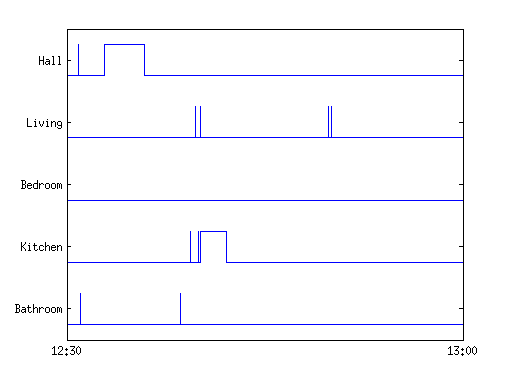
\includegraphics[width=\textwidth]{Pictures/FeatExample.png}
\label{fig:FeatEx}
\end{minipage}
\begin{minipage}{0.35\linewidth}
\centering
\begin{equation*}
 \begin{bmatrix} 
 o_{Hall}\\
 o_{Living}\\
 o_{Bedroom}\\
 o_{Kitchen}\\
 o_{Bathroom}
 \end{bmatrix}
 =
  \begin{bmatrix} 
 2\\
 4\\
 0\\
 3\\
 2
 \end{bmatrix}
\end{equation*}
\end{minipage}
\caption{Vector representation of the data. The data of the sensors is shown in the left image. It is translated in the vector shown on the right-hand side.}
\end{figure}

An additional dimension for the time is used. There are two different ways how the time dimension is added to the observations. The fine-grain representation adds the number of the time-slice in which an observations is captured, at the end of the observation vector. In the coarse-grain representation the 24 hours of a day are divided into the five time intervals $\{ 3am - 8am, 8am - 1pm, 1pm - 18pm, 18pm - 23pm, 23pm - 3am  \}$. So the observation of figure \ref{fig:FeatEx} will become $o_n=\{2,4,0,3,2,2\}$ in the coarse-grain representation. The observation falls into the second time interval. In the fine-grain representation the observation will be $o_n=\{2,4,0,3,2,20\}$ if the total number of time-slices on a day is $n=48$.

The given feature representation, with the two variation of the time dimensions, are used in the following chapters. But there are plenty more ways to describe the data so that it can be used in the LDA model. For example the size of the time-slices can be changed. This leads to a higher resolution and may give more detailed information of the behavior.
Another way to get a different feature representation is to combine sequential time-slices as it is described in the work of Farrahi et al. \cite{farrahi2008daily}. So for a given time-slice add the observation values of the previous and the subsequent time-slice. This will lead to a 15 dimensional observation plus one dimension for the time value. In this way the transitions are taken more into account, which might contain valuable information over the behavior.\\
We also might want to combine different sizes of time-slices into one observations, so that the global and detailed view is combined.\\
The different kind of sensor are also maybe important. The reed sensor, which is mostly installed at doors might contain more important information than the motion sensor. The motion sensor is also triggered by small movements, whereelse if a door is opened from a cupboard you can assume that an important action has taken place, as for example the person is grabbing a plate to prepare a meal. So it might be an idea to give a higher weight to sensor activities of reed sensors in house.\\
It is obvious that the feature space can be made nearly infinity big and it is quite a challenge to find the best feature representation. The likelihood that is gained from the EM-algorithms might be a good indication for a good feature representation.